\chapter{Présentation du projet}

\section{Hadoop et MapReduce}
{\it Hadoop}\cite{HadoopMapReduce} est une implémentation open source de {\it MapReduce} en Java distribuée par Apache.
 Les deux grandes parties de {\it Hadoop} sont :
\begin{itemize}
	\item {\bf Traitement des données} : Le framework {\it MapReduce}.
  	\item {\bf Stockage des données} : Hadoop Distributed File System. 
 \end{itemize}
 Le principe est de distribuer les données avec HDFS\footnote{Hadoop Distributed File System.} et de faire des traitements sur ces données là où elles sont stockées, grâce à {\it MapReduce}, afin de paralléliser des opérations.

{\it Hadoop} exécute une tâche de en commençant par diviser les données en entrée en blocs de données de même taille. Chaque bloc est ensuite planifié pour être exécuté.

\section{Contexte du projet}

Dans le cadre de notre projet de programmation, l'idée est de retranscrire la distribution des données en appliquant l'algorithme de {\it MapReduce} sans utiliser un framework\footnote{Le framework le plus connu pour {\it MapReduce} plus connu est {\it Hadoop}} ou un système de gestion de fichiers.

Le but est d'arriver à visualiser la simulation sur un cluster de machines.

\paragraph{Note}{\it Dans ce projet, il n'y a pas de cluster concret. Notre travail consiste seulement à simuler le comportement de {\it MapReduce} sur des machines fictives, indépendamment de tout matériel.}\\

La représentation graphique doit comprendre les phases de {\tt map()} et de {\tt reduce()}, toutes les deux fournies comme fonctions par l'utilisateur de l'application. Il faut pouvoir visualiser les connections qui existent entre {\tt map()} et {\tt reduce()} sur les différentes machines.\\

L'objectif du projet est de pouvoir déboguer facilement le code simulé.
Ces bogues peuvent correspondre à une mauvaise répartition des données dans l'ensemble du cluster qui sont invisibles pour l'utilisateur. En effet, le retour de l'exécution de {\it MapReduce} est un ensemble de paires clé/valeur et il n'est pas possible de savoir quel travail a été effectué par les processus. {\it VisualMapReduce} permet à l'utilisateur de voir si la quantité de machines et de cœurs de trop important par rapport à celle des données à traiter, et vis-versa.
Cette application, destinée à l'enseignement, permettra à des étudiants en Master 2 Informatique de simuler un cluster et comprendre le fonctionnement de {\it MapReduce}.

\section{Description détaillée de l'exécution de {\it MapReduce}}
\subsection{Notions importantes}

Avant de lister les différentes phases de {\it MapReduce}, rappelons les notions suivantes :

\begin{itemize}
\item {\bf Slot} : Le cluster d'exécution comprends $m$ machines avec $c$ coeurs, ce qui représente $m\times c$ slots d'exécution.
Un slot peut accueillir un {\it mapper} ou un {\it reducer}. Le slot est libéré lorsque l'exécution du {\it mapper} ou {\it reducer} se termine.
\item {\bf Job}  : Un job est un ensemble de {\tt map()} et {\tt reduce()}. Il dispose en entrée d'un jeu de données (Voir Figure \ref{fig:job}).
\begin{figure}[H]
  \centering
    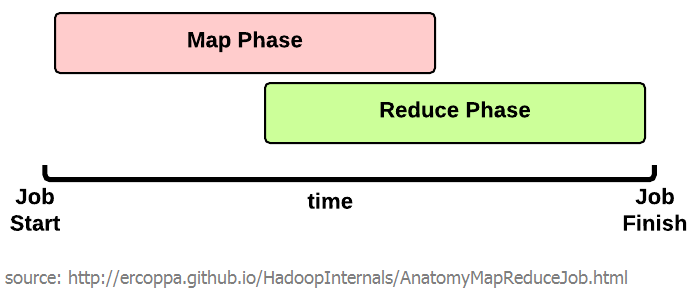
\includegraphics[width=0.75\textwidth]{images/job_timeline.png} 
        \caption{Job dans {\it MapReduce}}
    
\label{fig:job}
\end{figure}
\item {\bf Task} : On trouve des {\it MapTask} et des {\it ReduceTask}. Une phase de {\tt map()} comprend plusieurs {\it MapTask}, de même pour les phases de {\tt reduce()}.

\item {\bf Mapper/Reducer} : Ce sont les définitions des fonctions {\tt map()} et {\tt reduce()}. Un {\it mapper} est appliqué sur chaque slot. On a donc autant de {\it mapper} que de slots sur un le cluster\footnote{Il faut distinguer entre {\it mapper} et {\it MapTask}. Un {\it mapper} peut accueillir plusieurs {\it MapTask}. Une {\it MapTask} est une tache individuelle. Pour simplifier : $mapper = map+map+\ldots+map$}.\\
Le {\it mapper} est appliqué sur chaque entrée du résultat de la fonction de découpage {\tt split()} qui sera expliqué plus tard dans le document.  
Un {\it reducer} est appliqué sur toutes les valeurs associées aux mêmes clés générées.\\

Dans {\it MapReduce}, l'utilisateur définit un {\it mapper} et un {\it reducer} avec les signatures suivantes\cite{mapReduceTextProcessing}:
$$map: (k_1,v_1) \rightarrow [(k_2,v_2)]$$
$$reduce:(k_2,[v_2]) \rightarrow [(k_3,v_3)]$$
\end{itemize}

\subsection{Phases dans {\it MapReduce}}
L'algorithme {\it MapReduce} se décompose en plusieurs phases : {\bf Split}, {\bf Map}, {\bf Combine}, {\bf Partition}, {\bf Shuffle} et {\bf Reduce}.\\
\begin{itemize}
\item {\bf Split} : Récupère l'ensemble des données d'entrées et retourne des objets structurés qui serviront comme entrée de {\tt map()}. Dans la figure \ref{fig:mrwcp}, l'étape de {\tt split()} répartie un fichier textuel selon son nombre de lignes.

\item {\bf Map} : Prend en entrée une ou plusieurs données. Les résultats sont stockés sous forme de paires {\tt <key, value>}\footnote{<clé, valeur>} dites intermédiaires.

\item {\bf Combine}\footnote{La phase du {\it combine} n'était pas présent dans l'illustration qui a servi à la figure \ref{fig:mrwcp}. Nous l'avons modifié pour qu'elle y soit intégrée.} : {\it Optionnel.} Possède les mêmes propriétés d'entrée/sortie que {\tt map()}. Son but est de faciliter la tâche de reduce en efectuant un {\it merge} partiel\cite{Google} sur les résultats du {\tt map()}.\\

\item {\bf Partition} : Contrôle le partitionnement des clés des résultats de {\tt map()}. Par défaut, le {\it partitioner} utilise une fonction de hashage. Le nombre total de partitions est le même que le nombre des tâches de {\tt reduce()}. Le {\it partitioner} intervient entre les phases de {\tt map()} et {\tt shuffle()}. Pour l'exemple du {\it word count} de la figure \ref{fig:mrwcp}, il agit pour faire le partitionnement des sorties de {\tt map()} sur les 4 {\it reducer} qui existent.

\item {\bf Shuffle} : Phase de transfert des données des {\it mapper} aux {\it reducer}. Plus clairement, elle fournit les entrées de {\tt reduce()}.\\
Le {\tt shuffle()} est de la forme :
\[  shuffle:[(k_2,v_2)] \rightarrow (k_2,[v_2]) \]

\item {\bf Reduce}: C'est la phase de calcul du traitement. Elle accepte les clés intermédiaires et un ensemble de valeurs d'une même clé. Les valeurs sont alors traitées selon la fonction {\tt reduce()} fournie.\\
\end{itemize}

Pour mieux comprendre l'exécution de {\it MapReduce}, nous proposons l'exemple de {\it word count} qui compte le nombre d'occurrences des mots dans un texte. (Voir Figure \ref{fig:mrwcp})

\begin{figure}[H]
  \centering
    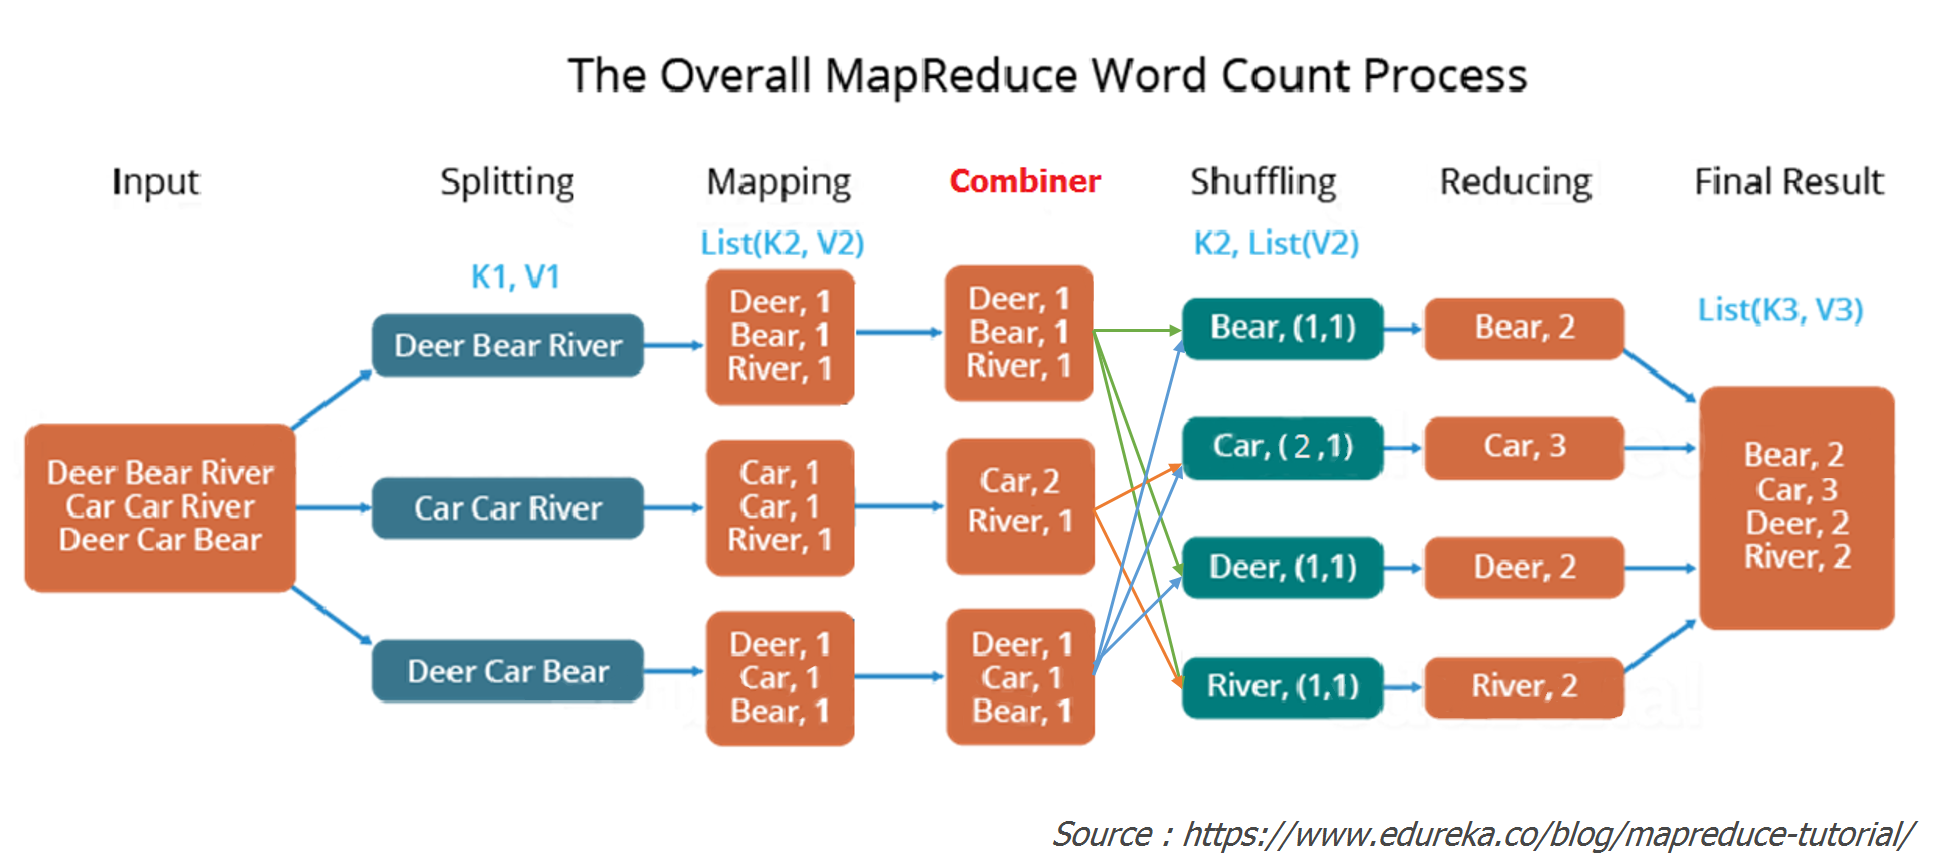
\includegraphics[width=1\textwidth]{images/mapreduce_process.png}
        \caption{Compteur d'occurrences de mots effectué par {\it MapReduce}}
          \label{fig:mrwcp}
\end{figure}
